\documentclass{sigchi}

% Use this command to override the default ACM copyright statement (e.g. for preprints). 
% Consult the conference website for the camera-ready copyright statement.


%% EXAMPLE BEGIN -- HOW TO OVERRIDE THE DEFAULT COPYRIGHT STRIP -- (July 22, 2013 - Paul Baumann)
\toappear{Copyright Eric Butler and Rahul Banerjee, 2014.}
%% EXAMPLE END -- HOW TO OVERRIDE THE DEFAULT COPYRIGHT STRIP -- (July 22, 2013 - Paul Baumann)


% Arabic page numbers for submission. 
% Remove this line to eliminate page numbers for the camera ready copy
\pagenumbering{arabic}


% Load basic packages
\usepackage{balance}  % to better equalize the last page
\usepackage{graphics} % for EPS, load graphicx instead
\usepackage{times}    % comment if you want LaTeX's default font
\usepackage{url}      % llt: nicely formatted URLs
\usepackage{color}
\usepackage{paralist}
\usepackage{subcaption}

% llt: Define a global style for URLs, rather that the default one
\makeatletter
\def\url@leostyle{%
  \@ifundefined{selectfont}{\def\UrlFont{\sf}}{\def\UrlFont{\small\bf\ttfamily}}}
\makeatother
\urlstyle{leo}


% To make various LaTeX processors do the right thing with page size.
\def\pprw{8.5in}
\def\pprh{11in}
\special{papersize=\pprw,\pprh}
\setlength{\paperwidth}{\pprw}
\setlength{\paperheight}{\pprh}
\setlength{\pdfpagewidth}{\pprw}
\setlength{\pdfpageheight}{\pprh}

\newcommand{\papertitle}{Visualizing Progressions for Education and Game Design}

% Make sure hyperref comes last of your loaded packages, 
% to give it a fighting chance of not being over-written, 
% since its job is to redefine many LaTeX commands.
\usepackage[pdftex]{hyperref}
\hypersetup{
pdftitle={\newcommand},
pdfauthor={LaTeX},
pdfkeywords={data visualization, game design},
bookmarksnumbered,
pdfstartview={FitH},
colorlinks,
citecolor=black,
filecolor=black,
linkcolor=black,
urlcolor=black,
breaklinks=true,
}

% create a shortcut to typeset table headings
\newcommand\tabhead[1]{\small\textbf{#1}}

\definecolor{Orange}{rgb}{1,0.5,0}
%\newcommand{\todo}[1]{\textsf{\textbf{\textcolor{Orange}{[[#1]]}}}}
\newcommand{\todo}[1]{}

% End of preamble. Here it comes the document.
\begin{document}

\title{\papertitle}

\numberofauthors{1}
\author{
  \alignauthor Eric Butler, Rahul Banerjee \\
   \affaddr{Center for Game Science}\\
   \affaddr{Department of Computer Science \& Engineering, University of Washington}\\
   \affaddr{\{edbutler,banerjee\}@cs.washington.edu} }

\maketitle

\begin{abstract}
Progression design is a critical part of designing games or educational content. Currently, systems to visualize the content of a progression are limited and do not help designers answer questions important to the design process. These questions include comparing two progressions to understand the relative order in which concepts are introduced or how complexity changes throughout the progression. We present an interactive visualization system that allows designers to compare two different progressions, using multiple views and interaction techniques that aim to help designers answer these questions. We evaluate our tool through informal anecdotes, discussing insights that were found on progression data for actively developed games.
\end{abstract}

\keywords{
	data visualization; game design;
}

\category{H.5.m.}{Information Interfaces and Presentation (e.g. HCI)}{Miscellaneous}

%See: \url{http://www.acm.org/about/class/1998/}
%for more information and the full list of ACM classifiers
%and descriptors. 

\section{Introduction}

A critical component of the design of educational or game experiences is crafting a coherent and effective sequence of content, called the \emph{progression}.
The progressions of skill-based games or educational curricula often aim to teach the player or student a series of different \emph{concepts}.
The design of progressions is a time-consuming, iterative process, where designers must carefully balance the ordering of concepts and how concepts are combined.
More recently, designers and researchers have attempted to create systems that can produce such content automatically (e.g., \cite{Andersen13}).
Understanding the structure of these progressions and their properties is crucial for effective design of either hand-crafted progressions or progression-generating algorithms, and visualization tools can aid the designer in this process.

One important task is comparing the quality of two different progressions.
Designs\todo{?} may be an in-development version of a game to a previous iteration, and deciding between two possible changes.
In research settings, when developing systems to automatically generate progressions, it can be beneficial, for example, to compare the output of the algorithm to a human-designed progression.
While there has been a lot of research into how to visualize player data~\cite{wallner2013visualization}, our task is slightly different:
we are focused on looking at the static design space of the game, without any player data.
There are several reasons designers may wish to analyze the design space of their game independent of player data.
Often, early in the design process, developers do not have access to player data, or such data is too expensive to gather.
There is value in getting ``first impressions'' of a design before putting it in front of players.
Likewise, when experimenting with automatic progression generation techniques, researchers should be able to have some understanding of their systems without first having to collect player data.
%Some people try to do static analysis without data~\cite{Jaffe12}.

However, there are few examples of such visualization systems, and such systems face several challenges.
We are concerned specifically with understanding the progression of \emph{concepts} that a player or student encounters in a skill-based game or piece of educational content.
Thus, \emph{progressions} are a sequence of \emph{stages} (e.g., problems, puzzles, levels, study units), where each stage covers a different set of concepts.
Both the number of concepts and number of stages may be high, in the dozens.
So a progression is a sequence of high-dimensional data, presenting challenges in visualization.
There are several activities we might want a useful progression comparison tool to support:
\begin{compactitem}
\item What is the order concepts are introduced in two different progressions?
\item How are particular concepts used in combination?
\item How does the complexity change over the progression?
\item How much of the ``design space'' is covered by one progression but not another; are there concepts or combinations that one of the progressions neglects?
\end{compactitem}

Little work exists in visualizing this specific domain.
Butler et al.\ visualize progressions as a table with stages on one axis and columns on the other \cite{Butler13}.
This visual encoding does not support answering all the questions we care to support, especially when the number of concepts or stages are large.
A good demonstration of how the table visualization fails to scale to a large number of stages/concepts can be found in Piotr Bugno's detailed outline of the story and puzzle progressions for \emph{Portal 2}\footnote{\url{http://www.piotrbugno.com/2012/06/portal-2-timelines/}}.
Though the ordering of concepts is clear, how they are combined is not, and viewing two of these charts together may yield little immediate insight as to their differences.

In this work we present a novel visualization system for comparing two different progressions to each other.
We evaluate its usefulness through informal, anecdotal case studies using datasets of progressions from the game \emph{Refraction}, an educational math game developed by our group.
We discuss insights provided by this visualization tool that are difficult to notice without it.

%Tools and visualizations specifically designed for the visualization and comparison of two different progressions are not well-studied.
%This is partially due to the fact that The existence is multiple progressions for a completed game is atypical. 
%However, recent research in the area of game design has created a need for such comparisons.
%Games may need to reach many different kinds of audiences and therefore may require different progressions for different populations \todo{cite}.
%For example, an educational math game may need to have a different difficulty curves for younger and older students.
%Other lines of research are attempting to design progression automatically~\cite{Andersen13,mandel2014offline}.
%Visualizations to help compare different algorithms to each other or human-designed progressions can aid researches in development of such algorithms.
%Even though final games often only have one progression, designers frequently go through several iterations of progressions during the development process based on user testing.
%Recent work on a tool to aid progression design suffered from a lack of useful visualizations for progressions~\cite{Butler13}.
%A lot of recent work has been trying to deal with progressions.
%Auto-generated progressions \cite{Andersen13}.
%Mixed-initiative progression designer \cite{Butler13}.
%People (we) have messed with static analysis tools \cite{Jaffe12}.

%Though the focus of this paper is on design on skill-based games, the progression design process also appears in creation of educational content.
%For example, choosing the sequence of concepts in a course curricula \todo{sub in whatever the paper actually said} is a form of progression design.
%\emph{Intelligent Tutoring Systems} (ITS) also rely on good progression design \todo{cite some stuff}.
%\todo{this para sucks, flesh it out}.

\section{Related Work}

The need to visualize sequences of values occurs in a wide range of other domains, such as stock market data or medical health records.
There exist several techniques for visualizing scalar values that vary over time, like line and bar charts~\cite{Playfair2005}.
When comparing multiple scalar values over time, stacked area charts and their variants work well~\cite{Havre2002}.
However, with higher-dimensional data (as ours is), effective visualizations must be created based on the semantics of the data.
In domains ranging from personal histories~\cite{Plaisant1996} to treatment plans~\cite{Kosara2001}, such visualizations have been designed by hand, based on the specifics of the domain.

Visualizing high-dimensional data is difficult, because most display surfaces are two-dimensional.
The use of 3D displays and/or animation can add at most two dimensions, but encoding the remaining dimensions in a visually perceptible way is challenging.
Several encodings for such data have been explored.
Some try to show all dimensions in the visualization.
The simplest method is to plot all values in a table, which allows the sequential nature of the data to be clearly shown.
However, some questions cannot be easily answered with tables, so we wish to supplement this view with other representations.
Multiple surveys on visualization of multidimensional data have been done~\cite{Wong1994,buja1996interactive}, while others survey visualization methods for time-dependent data~\cite{muller2003visualization}.
Chernoff faces~\cite{Chernoff73} attempt to encode several dimensions using parts of the human face.
It and related techniques, in addition to difficulty with accurate perception, do not scale to a large number of dimensions.
Parallel coordinates~\cite{Inselberg1991} plot the different dimensions on a set of parallel lines, using lines to connect particular datapoints across the dimensions.
However, parallel coordinates do not allow for the sequence to be easily represented with position encodings.
Another approach is to use dimensionality reduction techniques~\cite{Fodor2002}, sacrificing detail to increase interpretability. 
Linear methods for doing this include Principal Component Analysis (PCA)~\cite{dunteman1989principal}, Random Projections~\cite{baraniuk2009random}, etc., while non-linear methods include Kohonen's Self-Organizing Maps (SOM)~\cite{kohonen2001self}, and Multidimensional scaling (MDS)~\cite{kruskal1978mds}.
We use MDS in our tool, though other dimensionality reduction techniques could be explored in future work.

A related but distinct visualization problem is that of showing player data.
Current visualization systems geared towards helping game developers with the design process mainly target visualizing player data.
A recent survey describes several such systems~\cite{wallner2013visualization}.
Our system, in contrast, deals with data of a progression design space itself.
Sequences of player actions actually have a very similar structure to progressions: a player travels through a high-dimensional state space, and several systems aim to visualize this traversal in a 2D representation.
Researchers have found success using SOM (e.g., \cite{drachen2009player,thawonmas2006clustering}), MDS (e.g., \cite{Andersen10}), or other layout techniques (e.g., \cite{wallner2012spatiotemporal}).
However, one of our design requirements is to be able to drill down deeply into the set of concepts, for example, by looking at the ordering of concepts throughout the course of the progression.
While we can use some of these techniques for our problem domain, existing systems for looking at player data do not cover these use cases.

\section{System Description}

\subsection{Data Format}

Here, we describe our representation of \emph{progression} data, which are a sequence of stages and concepts associated with them.
Our system compares two progressions of a particular \emph{game}. The data provides a set of \emph{concepts}, $C = \{c_1, \ldots, c_m\}$, which represent various skills that appear in the game.
A progression is a sequence of stages $s_1, \ldots, s_n$,
each \emph{stage} $s_i$ described by a feature vector $s_i = \langle w_{i1}, w_{i2}, \ldots, w_{im} \rangle \in \mathbb{R}^m$, where $w_{ij}$ describes ``to what degree'' or ``how much of'' concept $c_j$ appears in stage $s_i$.

We assume that the set $C$ is semantically meaningful, such that differences in ``concept space'' correspond to differences in how players will experience the game. In particular, we assume that the Euclidean norm of the difference between two stages captures some useful aspect of how different two stages are with regards to their contents. The designer must produce such a set to use the visualization system.

\subsection{Refraction}

\begin{figure}[t]
\centering
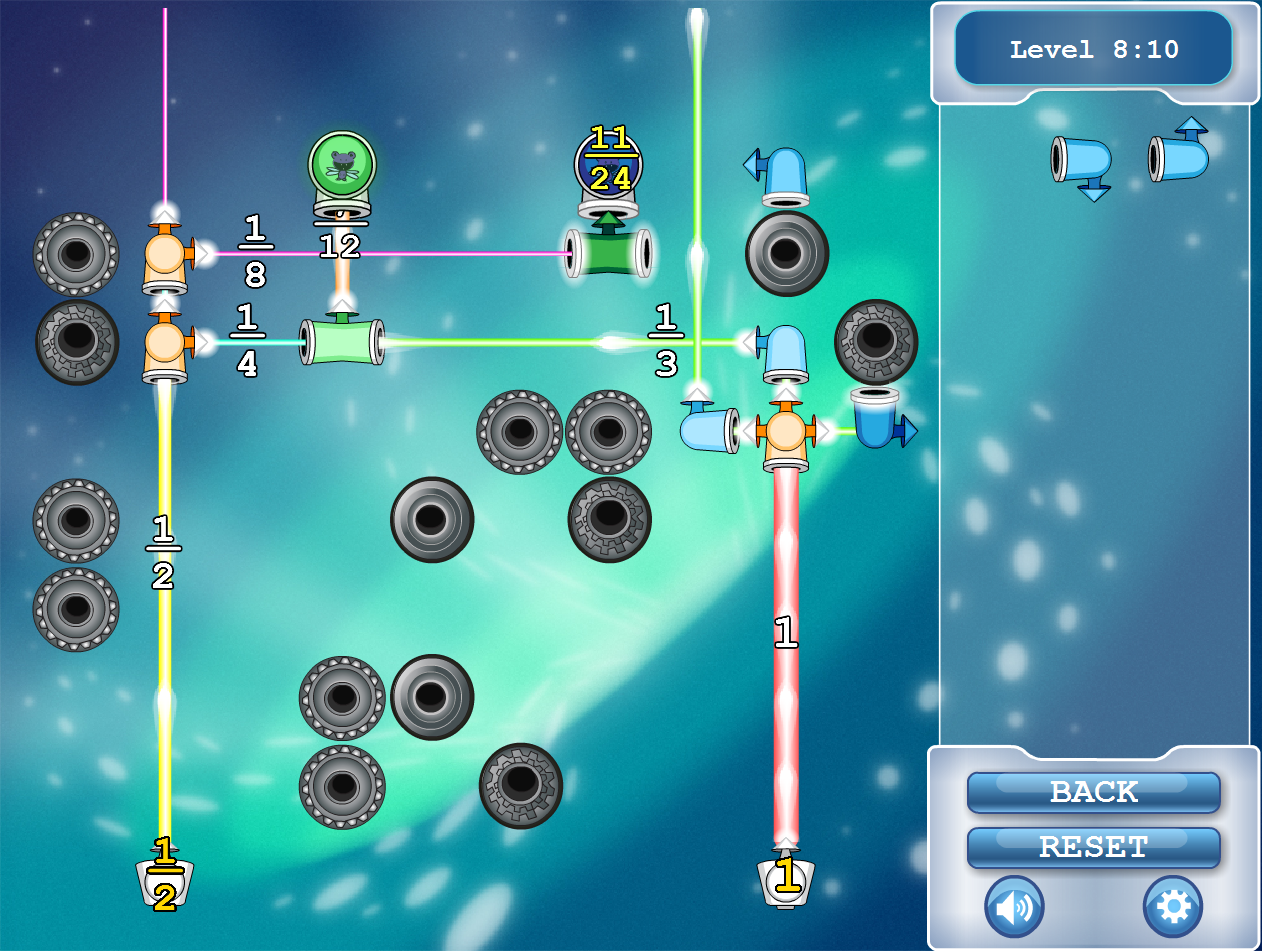
\includegraphics[width=\columnwidth]{images/refraction.png}
\caption{A stage of \emph{Refraction}, the game from which most of our datasets are drawn. We continue to develop new progressions for the game, hence the need for design tools. Most of the \emph{concepts} in \emph{Refraction} describe the various mathematical or spatial challenges in each puzzle.}
\label{fig:refraction}
\end{figure}

We first give a brief description of the particular game from which most of our examples are drawn, and use it to illustrate concrete examples of progression \emph{concepts}.
\emph{Refraction} is an educational puzzle game involving bending, splitting and combining lasers with fractional values.
It combines mathematical and spatial reasoning challenges.
A sample puzzle is shown in Figure~\ref{fig:refraction}.
Much of our research work involves or requires creating different progressions (both human-made and computer-generated) for \emph{Refraction} and other games, which is a primary reason tools to compare progressions would be useful (e.g., \cite{Butler13,orourke2013effects,orourke2014brain,Andersen12,mandel2014offline}).

\emph{Concepts} in the game describe the various mathematical and spatial challenges of each puzzle.
For example, the ``\texttt{num\_splitter}'' concept describes how many \emph{splitter pieces}, pieces that split lasers into equal fractional parts, must be used to solve the puzzle.
The concept ``\texttt{source\_power\_fraction}'' describes whether \emph{source pieces}, the pieces from which the lasers originate, emit lasers with fractional values or integer values.
The datasets have two alternative concept sets; one is a full set of approximately 60 binary concepts, and the other is a set where those 60 concepts are collapsed into around 15 integer-valued categories.
Other games have their own concept sets specific to their mechanics and rules.

\subsection{Interface}
Our system provides three different views of progression data, and interactive controls for manipulating these views.

\begin{figure}[t]
\centering
\begin{subfigure}[b]{0.45\textwidth}
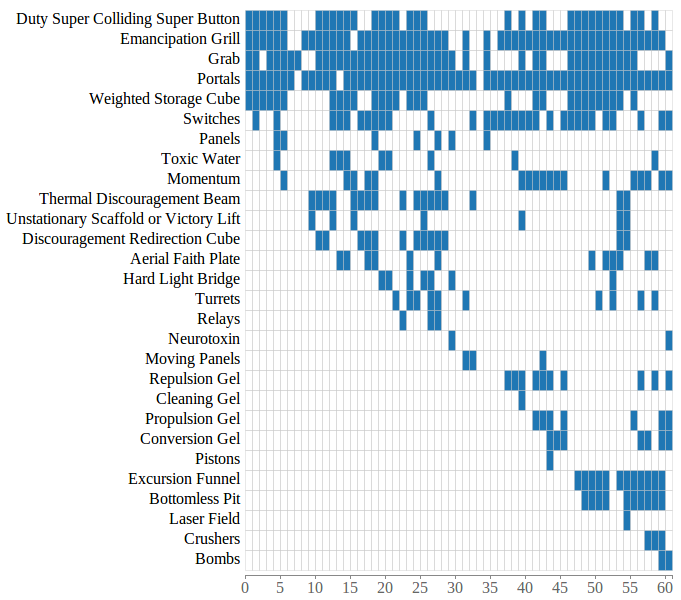
\includegraphics[width=\columnwidth]{images/portal_grid_view.png}
\caption{Portal 2}
\label{fig:portal_grid_view}
\end{subfigure}
\begin{subfigure}[b]{0.45\textwidth}
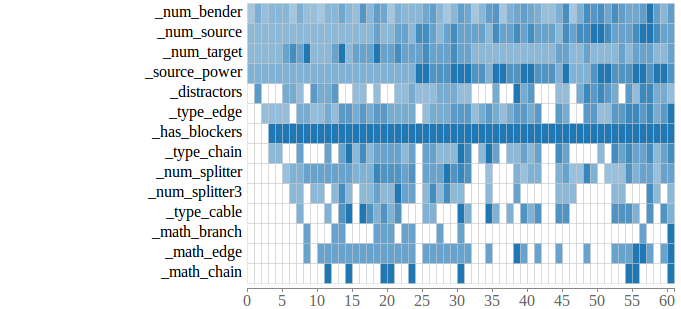
\includegraphics[width=\columnwidth]{images/refraction_original_collapsed.png}
\caption{Refraction}
\label{fig:refraction_grid_view}
\end{subfigure}
\caption{Concept progressions for (a) Portal 2 and (b) Refraction displayed as grids.}
\label{fig:grid_view}
\end{figure}

The \emph{grid} is a table with concepts mapped to rows and stages mapped to columns.
The cell for a particular stage and concept represents how much that concept is used in that stage (higher counts map to more saturated color).
Figure~\ref{fig:grid_view} shows grid views for concept progressions from two different games (Refraction and Portal 2).
When viewing the grid, our system lets the user sort the rows (concepts) according to their order of appearance in the progression.
Thus, the concept introduced first in the progression is on the top row, and the one introduced last is assigned the last row.
The rows can also be ordered alphabetically (by concept name), or they can simply reflect the ordering in the data source.

The \emph{projection} view shows MDS projections for progressions, computed using the SMACOF (Scaling by Majorizing a Complicated Function) method~\cite{De2011}.
Feature vectors from each stage are projected into 2 dimensions, which are mapped to position.
Every stage is rendered as a node, and nodes corresponding to adjacent stages are connected via edges.
Multiple progressions are drawn in the same 2D region, rendered with transparency to mitigate occlusion caused by overlaps.

The user can also select a particular set of concepts and ``drill down'' to see how their occurrences vary precisely over various stages by selecting them in the ``Filter To:'' control.
When one or more concepts are selected in the filter, our system shows \emph{bar charts}, one chart per concept.
Concept occurrence is mapped to bar height, while the horizontal axis represents different stages.
When no concepts are selected (or the ``Clear Filters'' button is clicked), the bar charts are hidden and the grid view is shown.

Brushing is supported inside all views by clicking and dragging to specify a rectangular region, which selects all elements inside its extents.
Selection changes an element's color to red.
Linking ensures that brushing inside the grid, bar chart or projection view automatically selects the corresponding elements in the other visible views.

\begin{figure*}[t]
\centering
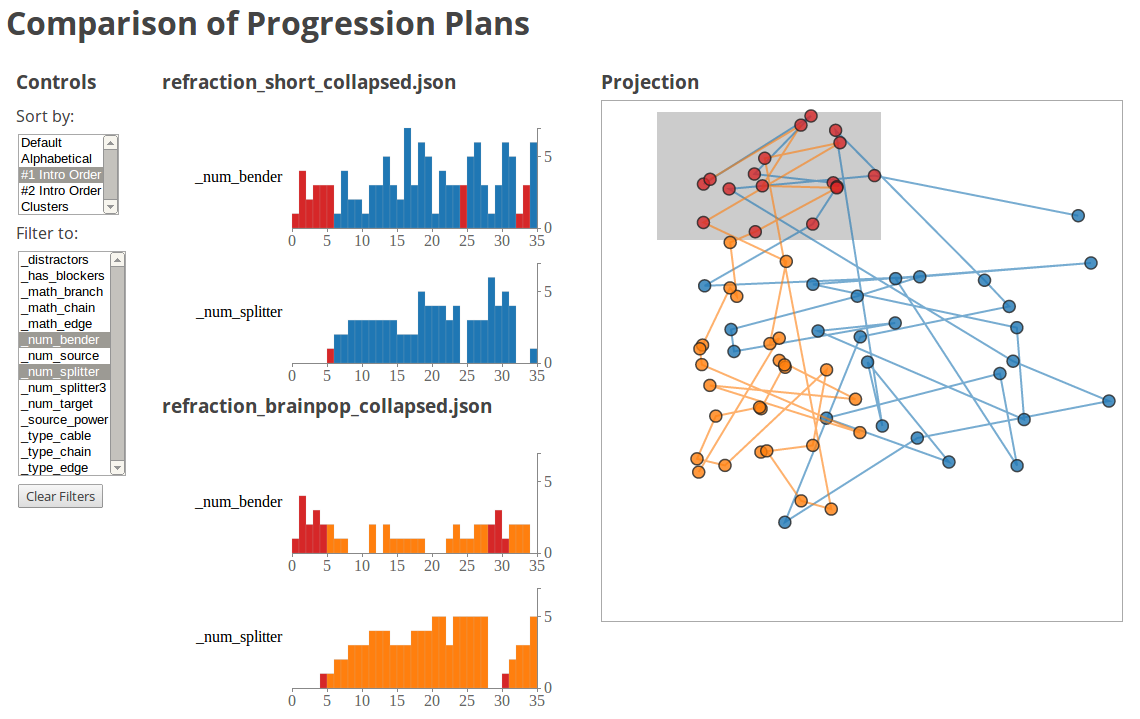
\includegraphics[width=2\columnwidth]{images/full_screenshot.png}
\caption{A screenshot of our system's interface, showing its filtering, brushing and linking capabilities. Here, on the left is a detailed view of two particular concepts for each progression, while the right shows the MDS projection of both progressions onto a 2D plane.}
\label{fig:full_screenshot}
\end{figure*}

Figure~\ref{fig:full_screenshot} shows a screenshot of our system being used to compare two progressions for Refraction.
On the left are sorting controls (used for ordering the rows in the bar chart), and filters below (to select particular concepts for inspection).
Here, two concepts (``\texttt{num\_bender}'' and ``\texttt{num\_splitter}'') are selected.
In the center are bar charts showing the concept occurence counts for the selected concepts (one set of bar charts per progression).
On the right, we see the MDS projection for both progressions, with some nodes selected via brushing, and corresponding nodes in the bar charts selected via linking.

\section{Discussion}

In this section we discuss anecdotes of insights made possible through use of this tool as well as limitations of the system.

\begin{figure}[t]
\centering
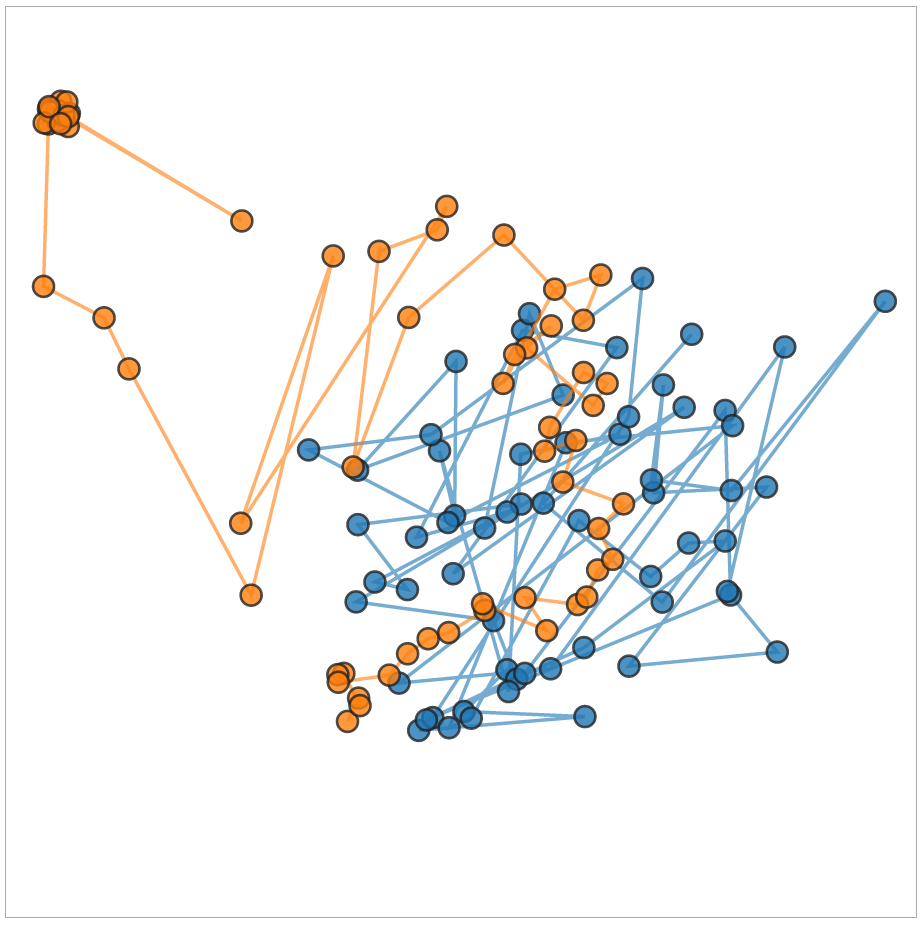
\includegraphics[width=\columnwidth]{images/mds_original_generated.png}
\caption{A human-crafted progression (blue) and one of our attempts at an automatically-generated progression (orange). The MDS projection clearly illustrates some of the qualitative differences between the two progressions.}
\label{fig:mds_original_generated}
\end{figure}

Recent research efforts in our group have attempted to create progressions (for games such as \emph{Refraction}) automatically.
One goal of these algorithms was to replicate the success of the human-designed progressions,
and one approach is to try to create progressions with the same basic structure as human-designed ones.
When creating these algorithms, the best tools we had were manual inspection by playing through the game or looking at tables of computed features.
However, when a computer-generated and a human-designed progression were compared in our tool, certain strong differences were immediately apparent.
Figure~\ref{fig:mds_original_generated} shows the MDS projection of two progressions: blue is human, orange is computer.
It is clear that the successive stages in the computer progression are very close in ``concept space,'' whereas the human progression moves much more chaotically through the space.
This leads us to infer that the computer-created progression does not have enough variance from one puzzle to the next.
Another interesting feature that is immediately obvious is that the computer progression eventually gets stuck and gives essentially very similar puzzles 20 times in a row.

\begin{figure}[t]
\centering
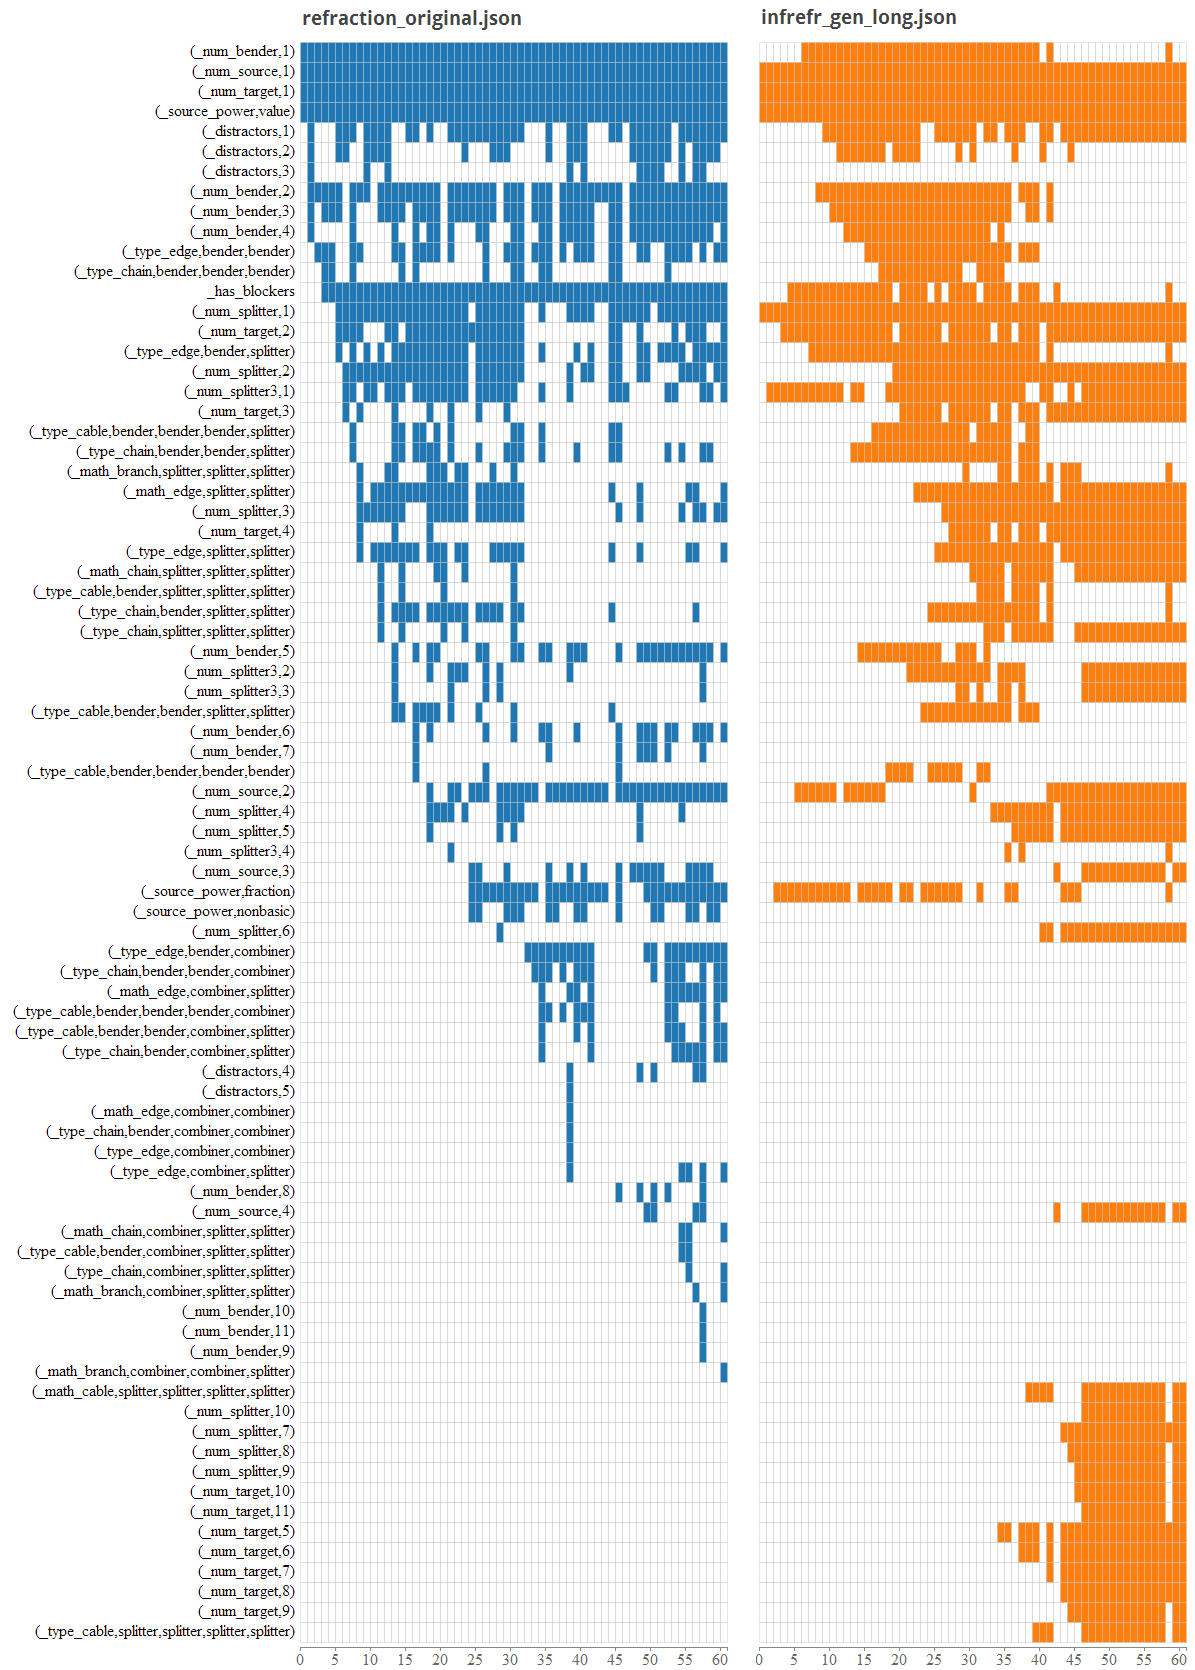
\includegraphics[width=\columnwidth]{images/ordering_orig_gen.png}
\caption{Comparing ordering of concepts between human-crafted (blue, on left) and computer-generated (orange, on right) progressions. The concepts are sorted by introduction order of the left progression, making differences in ordering between the two datasets apparent. Note that while typically this grid view uses hue to show quantitative values for each concept, this particular concept set is all binary. This screenshot is cropped for display purposes; the tool shows it slightly differently.}
\label{fig:ordering_orig_gen}
\end{figure}

Another measure on which we want to compare the progressions is ordering of concepts.
The tool allows us to easily sort one progression by the ordering of another, in order to make differences readily apparent.
This is illustrated in Figure~\ref{fig:ordering_orig_gen}, where we compare the same progressions by ordering.
Here, we use a very detailed breakdown on the concept space.
We immediately notice several concepts that appear very early in the computer-generated progression but very late in the human-generated progression.
Additionally, we can clearly see how the games diverge in the later half of the progression. The sets of concepts introduced in the second half of each progression are nearly disjoint.

\subsection{Limitations}

One significant limitation in the system is that it relies on the concept set to be semantically meaningful so that operations such as taking the Euclidean distance between stages is sensible.
This is obviously a tall order for game designers to satisfy before they can use the tool, as it is not clear which concepts actually affect player experience without testing.
One possible remedy for this is to explore unsupervised machine learning techniques to deduce more meaningful concept dimensions, perhaps by clustering or dimensionality reduction techniques.
If this tool were being used in a later stage of development when player data from user tests are available, that could be used in such an analysis by trying to learn which particular concepts have measurable impact on player experience.
Another approach would be to allow the designer to interactively organize and categorize concepts while exploring with the tool, rather than beforehand.

Another major problem is the lack of a significant number of datasets for this domain.
Though we believe this will change in the future, currently, explicitly creating data representations of progressions is rare and limited primarily to a small set of research groups.
While we can (and did) manually create datasets for existing games, games very rarely have multiple progressions in final versions, as multiple progressions often only appear during iteration in the development process.
On the other hand, while educational domains very frequently have wildly different progressions for a particular domain (e.g., high-school algebra), formal representations of these progressions for use in visualization are very rare.
Therefore, though we believe these activities can be generally applicable to a wide range of games or educational domains, it is difficult to substantiate such a claim without other datasets on which to evaluate the tool's generality.

A minor limitation of our system is that it currently does not scale gracefully to extremely long progressions.
While progressions with around 100 stages display quickly, computing MDS on significantly longer progressions takes more time, increasing the latency before being able to interact.

\section{Conclusion}

We have presented a system that aims to help designers compare and answer important design questions about progressions during the design process.
The tool supports several different encodings of progression data such as tables and MDS projections, supporting answering questions about things such as the ordering of introduction of concepts or how two different progressions move through the design space.
Anecdotal evidence suggests that this tool can be useful in providing insight to designers.

There are several avenues of future work, in addition to overcoming previously mentioned limitations.
We only used one dimensionality-reduction technique; others should be explored to find more effective ones.
Though our system is designed for use where player data is not available, it could be improved in cases where such data does exist by integrating visualizations of such data into the tool. For example, the tool could allow designers to drill down into a particular stage and view statistics on how players performed on that stage, or aggregate statistics about each stage could be displayed alongside the table. Though this system was designed for a research setting, industry developers could likely benefit from such a tool, and a more thorough evaluation of the requirements for such a tool could be conducted.
This system supports linear sequences; however, several professional or research games or educational systems use non-linear progression structures, for example by choosing the next math problem based on performance of the student. Techniques to better understand these structures could be explored.

% make the last page all pretty like:
% hack, if necessary:
% http://stackoverflow.com/questions/2149854/how-to-manually-equalize-columns-in-an-ieee-paper-if-using-bibtex
% Or, just remove \balance and give up on balancing the last page.
%\balance

\bibliographystyle{acm-sigchi}
\bibliography{biblio}
\end{document}

